% Please do not change the document class
\documentclass{scrartcl}

% Please do not change these packages
\usepackage[hidelinks]{hyperref}
\usepackage[none]{hyphenat}
\usepackage{setspace}
\doublespace

% You may add additional packages here
\usepackage{amsmath}
\usepackage{graphicx}
\usepackage{wrapfig}
\graphicspath{ {./images/} }
\usepackage{multirow}
\usepackage[rightcaption]{sidecap}

% Please include a clear, concise, and descriptive title
\title{Comp140 Usability Analysis} 

% Please do not change the subtitle
\subtitle{Comp140 Usability Analysis}

% Please put your student number in the author field
\author{1507516}

\begin{document}

\maketitle

\abstract{}

\section{Game controller and Evaluation}

The game controller was a minimalist design because the controls for the game were fairly simple. The design was inspired by the Wii nunchuck and the razer hydra. It featured directional buttons, and a trigger button at the end which made the player attack. The controller went through a few iterations before coming to it's final design. The initial design was made out of play-dough and had a lot of issues due to the play-dough being conductive. For the second sprint the controller was re-designed out of cardboard and paper, with electrical paint for the directional arrows, and play-dough for the trigger button.





\section{Heuristics by Jakob Nielsen\cite{nielsen1990heuristic}}
\subsection{Aesthetic and minimalist design:}

The controller aesthetic is simple and contains no extra information which is needed by the user, as most of the design is following typical standards that are familiar to the user and thus, no extra information is required. 

\subsection{Match between system and the real world:}

The design of the controller is shaped in a way that it uses familiar concepts, such as a hand grip that would fit into the hand easily, thus prompting the user to hold the controller by the grip.

\subsection{Recognition rather than recall:}

The controller has a few key features that are recognizable to the user, such as a grip to hold the controller by, and directional arrows that need to be pressed by the user. Furthermore when the user holds the controller their finger naturally curves round the top and over the kick button.

\section{Recommended improvements}

\subsection{Improvement one:}
The controller requires more ergonomic design as the design was too hard to hold and press the button at the end. This could of been done by reducing the length of the controller so that players with small hands could reach the end button easily. Furthermore the button also was not satisfying to press as it was very flimsy and moved about when it as pressed because it was only attached by a metal wire. This could of been improved by attaching the button to the controller and making it more robust.

\subsection{Improvement two:}
Another button was needed for the block mechanic, although with the version of the game I was working with did not have a working block mechanic, this would of been needed for the final version of the game where it did work.

%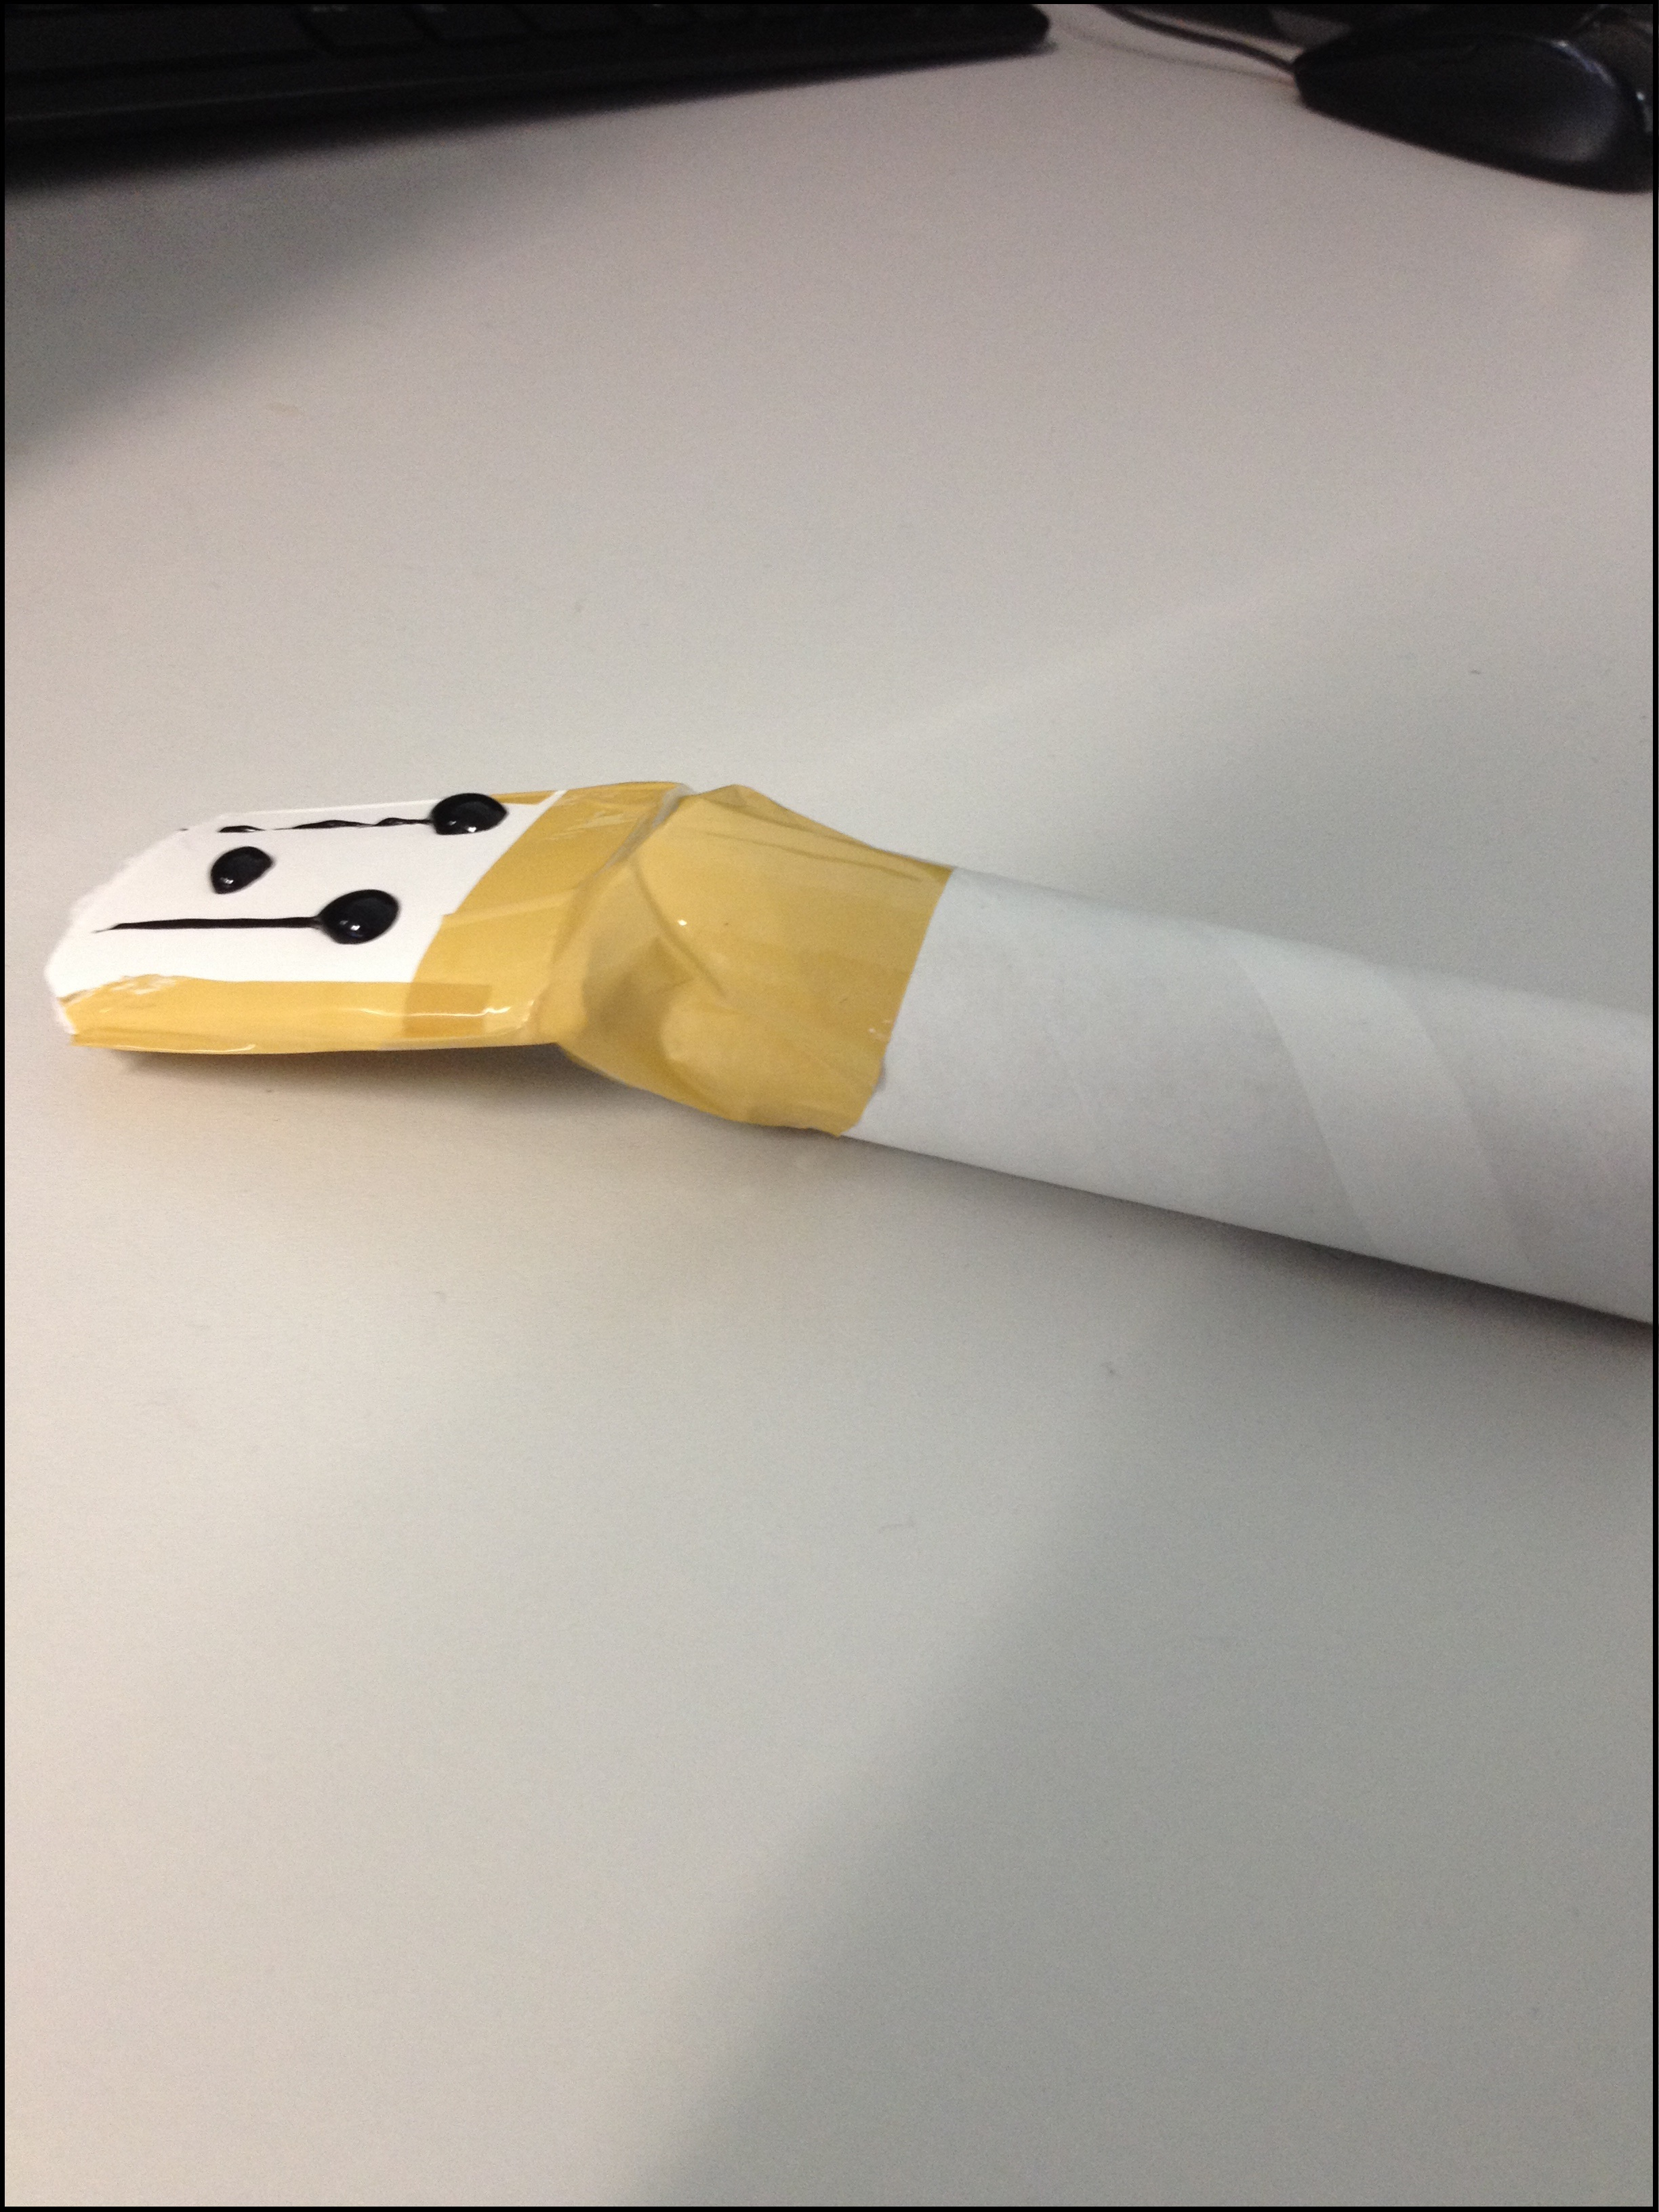
\includegraphics[width=\textwidth]{Final-Design}

\begin{figure}[h]
\centering
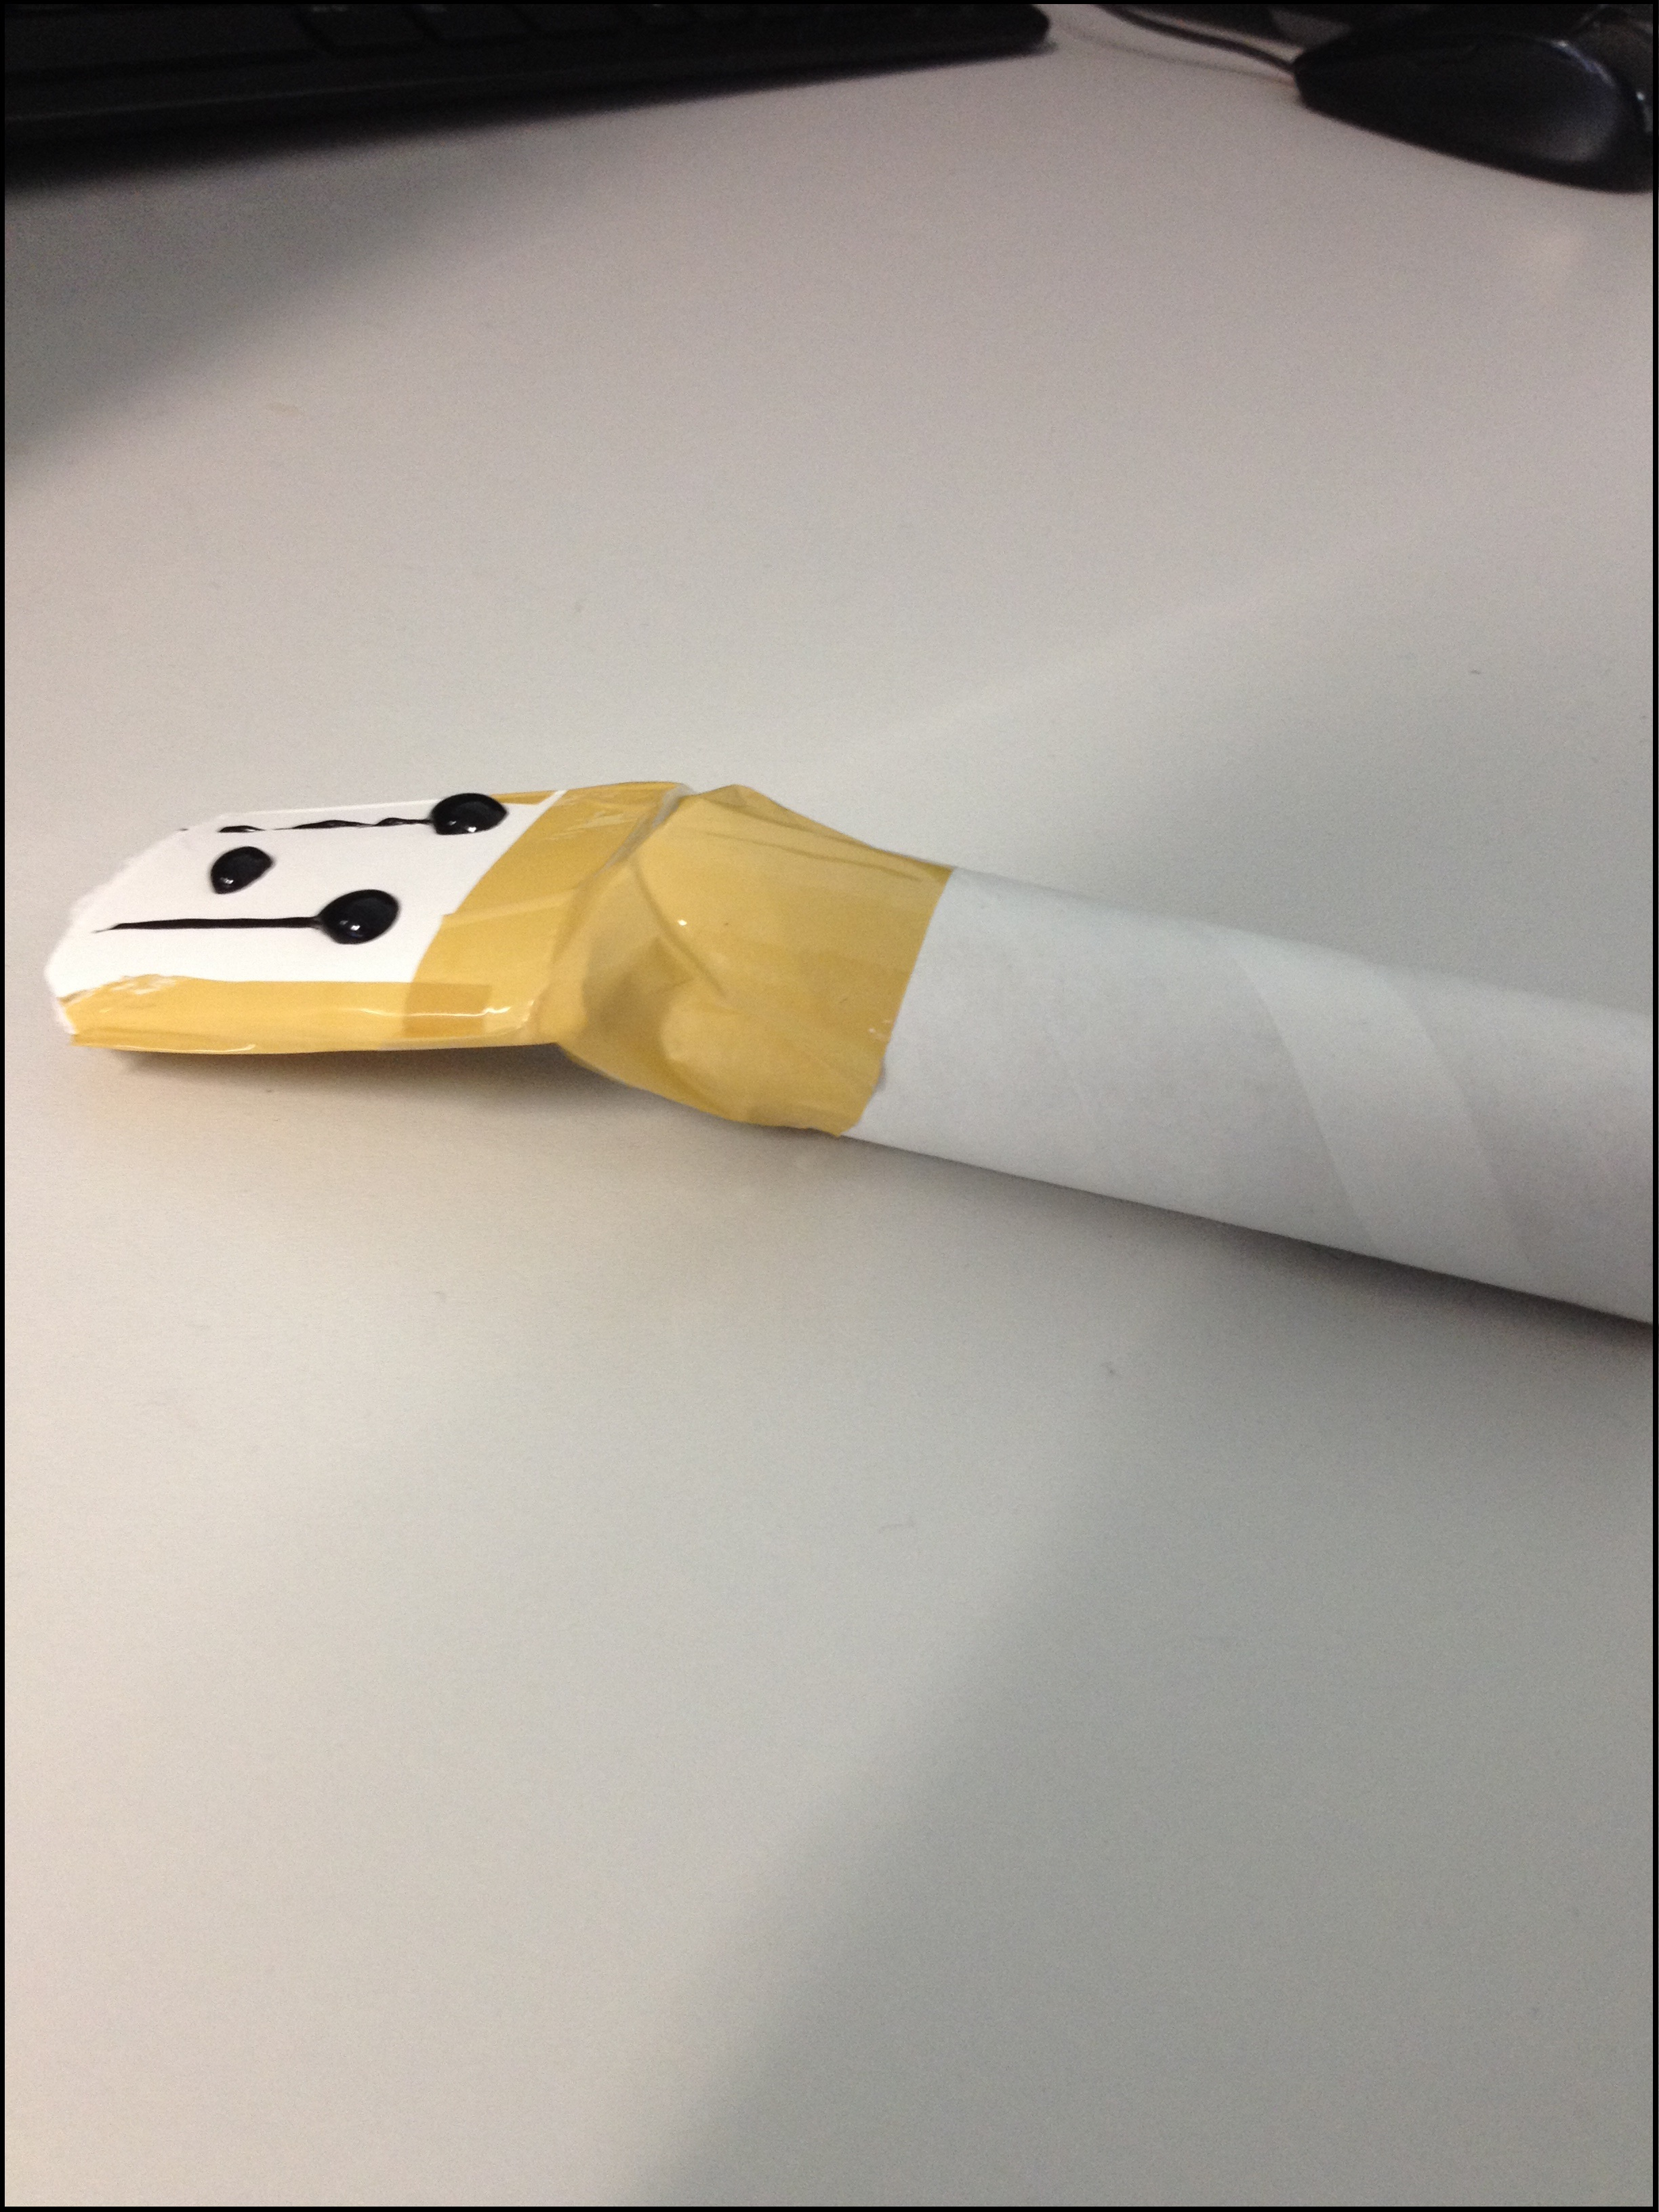
\includegraphics[width=0.5\textwidth]{Final-Design}
\caption{Final Prototype Controller Design}
\end{figure}


\section{Conclusion}

If I was to re-design the controller I would have changed the size of the controller and use a different material that is more sturdy. I would of also added another button at the bottom of the controller so the player could block the attacks.

\bibliographystyle{ieeetr}
\bibliography{comp140_Usability}

\end{document}
